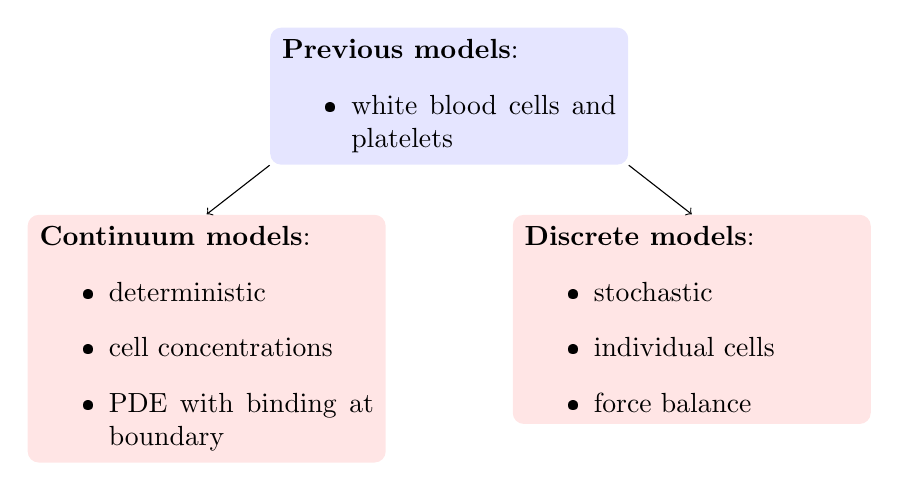
\begin{tikzpicture}
  \node (root) at (0, 0)
  [rounded corners, fill=blue!10, inner sep=1ex]
  {
    \begin{minipage}{.35\linewidth}
      \textbf{Previous models}: 
      \begin{itemize}
      \item white blood cells and platelets
      \end{itemize}
    \end{minipage}
  };
  
  \node (left child) at (-.8, -1.5)
  [below left, rounded corners, fill=red!10, inner sep=1ex]
  {
    \begin{minipage}{.35\linewidth}
      \textbf{Continuum models}: 
      \begin{itemize}
      \item deterministic
      \item cell concentrations
      \item PDE with binding at boundary
      \end{itemize}
    \end{minipage}
  };
  
  \node (right child) at (.8, -1.5)
  [below right, rounded corners, fill=red!10, inner sep=1ex]
  {
    \begin{minipage}{.35\linewidth}
      \textbf{Discrete models}: 
      \begin{itemize}
      \item stochastic
      \item individual cells 
      \item force balance
      \end{itemize}
    \end{minipage}
  };

  \draw[->] (root.south west) -- (left child.north);
  \draw[->] (root.south east) -- (right child.north);
\end{tikzpicture}
